\documentclass{beamer}
\usepackage{pgfpages}
\usepackage[backend=bibtex]{biblatex}
\usepackage{multicol}
\usepackage{multimedia}
\usepackage[absolute,overlay]{textpos}
\usepackage{parskip}
\usepackage{hyperref}
\usepackage{lmodern}
\usepackage{bbding}
\usepackage[absolute,overlay]{textpos}
\usepackage{framed} %Used to shade important equations, color devined with shadecolor
\hypersetup{colorlinks=true, urlcolor=blue}
\setlength{\parskip}{\smallskipamount}
\colorlet{shadecolor}{cyan}
%\usepackage[texcoord,grid,gridunit=mm,gridcolor=red!10,subgridcolor=green!10]{eso-pic} %DELETE when done with grid
\setbeameroption{hide notes} % Only slides
%\setbeameroption{show only notes} % Only notes
%\setbeameroption{show notes on second screen=right} % Both
%\bibliography{../../papers/references.bib}
\setbeamerfont{footnote}{size=\tiny}
%\AtEveryCitekey{\clearfield{title}}

%
% Choose how your presentation looks.
%
% For more themes, color themes and font themes, see:
% http://deic.uab.es/~iblanes/beamer_gallery/index_by_theme.html
%
\mode<presentation>
{
\usetheme{Warsaw}      % or try Darmstadt, Madrid, Warsaw, ...
\usecolortheme{default} % or try albatross, beaver, crane, ...
\usefonttheme{default}  % or try serif, structurebold, ...
\setbeamertemplate{navigation symbols}{}
\setbeamertemplate{caption}[numbered]
} 

\usepackage[english]{babel}
%\usepackage[utf8x]{inputenc} %Doesn't play well with biblatex
\usepackage{amssymb}
\usepackage{bm}
\usepackage{color}
\usepackage{graphicx}
\setbeamercovered{invisible}
\setbeamercovered{%
again covered={\opaqueness<1->{100}}} %This changes the opaqueness of each bullet

\newcommand{\red}[1]{{\color{red}{#1}}}
\newcommand{\checkH}[2]{\begin{textblock*}{1cm}(#1,#2){\Huge \red{\Checkmark}}\end{textblock*}}
\newcommand{\checkh}[2]{\begin{textblock*}{1cm}(#1,#2){\huge \red{\Checkmark}}\end{textblock*}}
\newcommand{\checkL}[2]{\begin{textblock*}{1cm}(#1,#2){\Large \red{\Checkmark}}\end{textblock*}}
\newcommand{\checkl}[2]{\begin{textblock*}{1cm}(#1,#2){\large \red{\Checkmark}}\end{textblock*}}
\renewcommand{\rm}[1]{\mathrm{#1}}

\title[{\color{white}{Chapters 2.2-4}}]{Physics 121: \\ Instantaneous Velocity, Kinematic Equations}
\author{Cody Petrie}
\institute{Mesa Community College}
\date{}

\begin{document}

%\setbeamertemplate{frametitle}[default][center]
\begin{frame}
\titlepage
\end{frame}

% Uncomment these lines for an automatically generated outline.
%\begin{frame}{Outline}
%  \tableofcontents
%\end{frame}

% Commands to include a figure:
%\begin{figure}
%\includegraphics[width=\textwidth]{your-figure's-file-name}
%\caption{\label{fig:your-figure}Caption goes here.}
%\end{figure}

\begin{frame}{Quiz}
\begin{enumerate}
   \item True/False: If an object has a negative acceleration it must be slowing down. \\~\\
   \item What is the velocity of the object whose x(t) graph is shown below? Don't just write it, explain {\bf briefly} how you got it.
\end{enumerate}
\begin{center}
   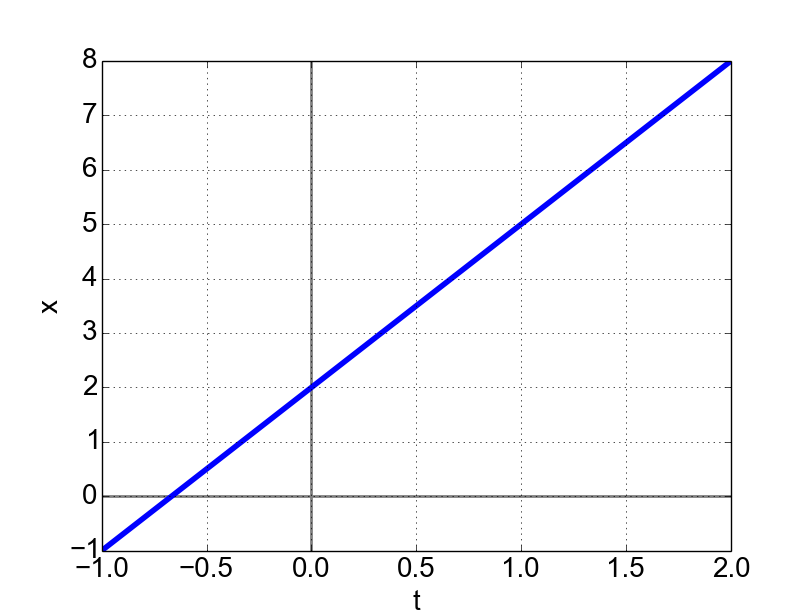
\includegraphics[width=0.7\textwidth]{../figures/2_2-4Quiz.png}
\end{center}
\end{frame}

\begin{frame}{Questions}
\begin{center}
   \color{blue}{\Huge How is HW going?}
\end{center}
\end{frame}

\begin{frame}{Instantaneous Velocity}
\begin{itemize}
   \item<1-> Instantaneous and average velocities are slightly different. Which is displayed on the speedometer of your car?
   \begin{itemize}
      \item<2-> Instantaneous velocity
   \end{itemize}
   \item<3-> Let's try to illustrate the difference and when it's appropriate to use average velocities.
\end{itemize}
\begin{center}
\uncover<3>{
~\\ This is an accelerating rocket (not uniform motion anymore)
   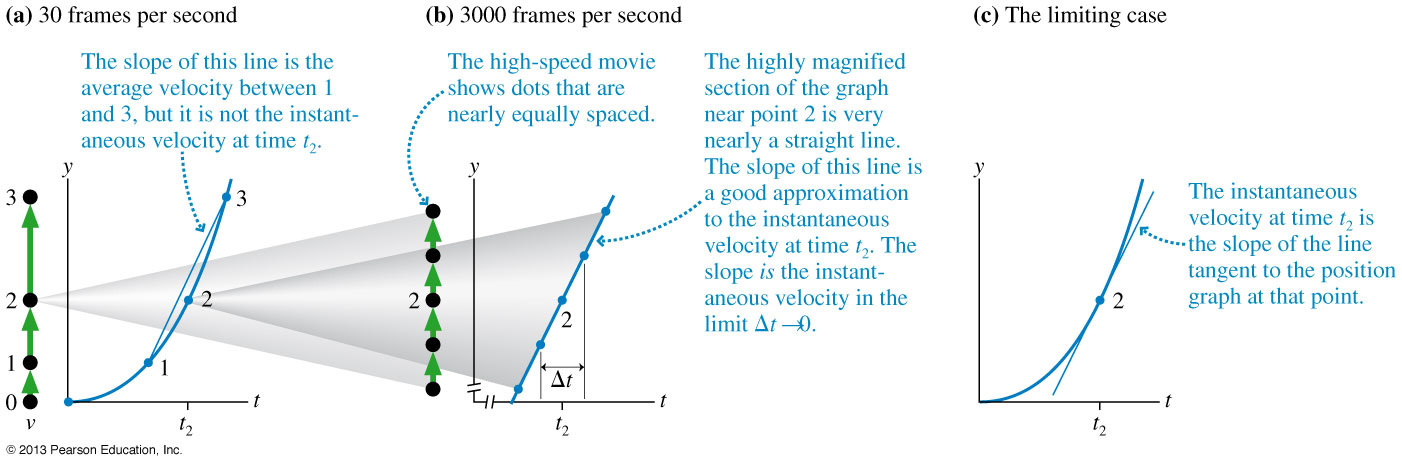
\includegraphics[width=\textwidth]{../figures/02_09_Figure.jpg}
}
\end{center}
\end{frame}

\begin{frame}{Quick Check}
\begin{center}
   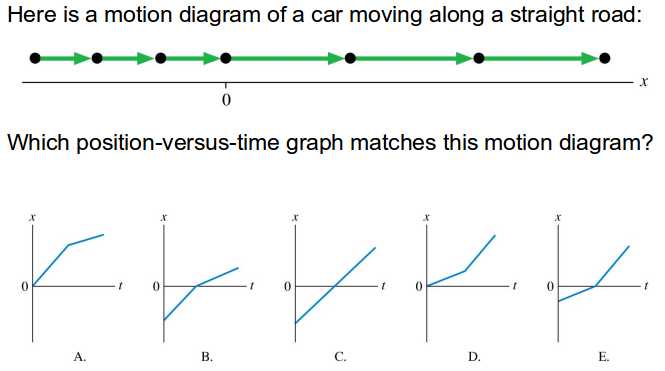
\includegraphics[width=\textwidth]{../figures/QC2_3.png}
\end{center}
\only<2->{\checkh{10.7cm}{7.2cm}}
\end{frame}

\begin{frame}{Quick Check}
\begin{center}
   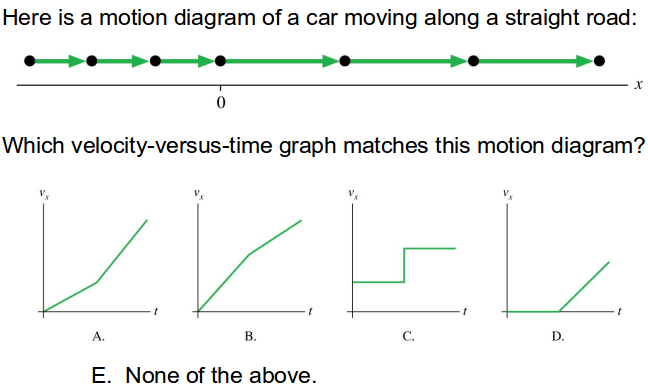
\includegraphics[width=\textwidth]{../figures/QC2_4.png}
\end{center}
\only<2->{\checkh{7.5cm}{7.0cm}}
\end{frame}

\begin{frame}{Quick Check}
\begin{center}
   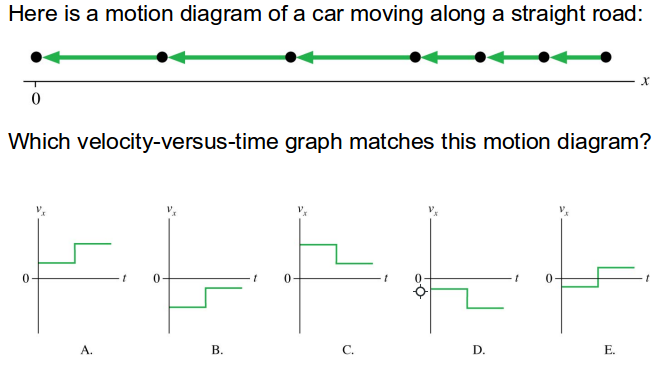
\includegraphics[width=\textwidth]{../figures/QC2_5.png}
\end{center}
\only<2->{\checkh{8.6cm}{7.3cm}}
\end{frame}

\begin{frame}{Instantaneous Velocity}
\begin{itemize}
   \item As you zoom in more and more on the graph it's like taking smaller and smaller $\Delta t$ steps. The truly instantaneous velocity is when you take $\Delta t \rightarrow 0$.
   \begin{shaded}
   \begin{align*}
      v_s \equiv \lim\limits_{\Delta t \rightarrow 0} \frac{\Delta s}{\Delta t} = \frac{ds}{dt} ~~~~~ \text{(Instantaneous Velocity)} \\
      v_s = \text{slope of the position-versus-time graph at time $t$}
   \end{align*}
   \end{shaded}
   \item<2-> If v is the slope of x(t) then how to we get x from v(t)?
   \begin{itemize}
      \item<3-> Some of you might recognize that as an integral.
   \end{itemize}
\end{itemize}
\uncover<3>{\begin{center}\begin{equation}
   x(t) = \int v(t)dt + x_0
\end{equation}\end{center}}
\end{frame}

\begin{frame}{Derivatives Review}
\begin{itemize}
   \item $\frac{ds}{dt}$ is called {\it derivative of s with respect to t}.
   \item The derivative is the slope of the line that is tangent to the to the position vs. time graph.
   \item The book (and probably I) will only deal with derivaties of powers and polynomials so let's review those.
\end{itemize}
\end{frame}


\begin{frame}{Derivatives Review}
\begin{center}
   If $u(t)=ct^n$ then $\frac{du}{dt} = \uncover<2>{nct^{n-1}}$
   \uncover<3>{\\~\\ Let's try this with a specific example then. Let the trajectory of the particle be $s(t) = 2t^2$. Now solve for the velocity of the particle at any time along the path.
   \begin{equation*}
      \frac{ds}{dt} = \uncover<4>{4t}
   \end{equation*}}
\end{center}
\end{frame}

\begin{frame}{Derivatives Review}
\begin{center}
   Here are a couple more that might be usesful to remember.
   \begin{equation*}
      \frac{d}{dt} \text{C} = \uncover<2>{0}
   \end{equation*}
   \begin{equation*}
      \frac{d}{dt} (u(t)+w(t)) = \uncover<2>{\frac{du}{dt}+\frac{dw}{dt}}
   \end{equation*}
\end{center}
\end{frame}

\begin{frame}{Quick Check}
\begin{center}
   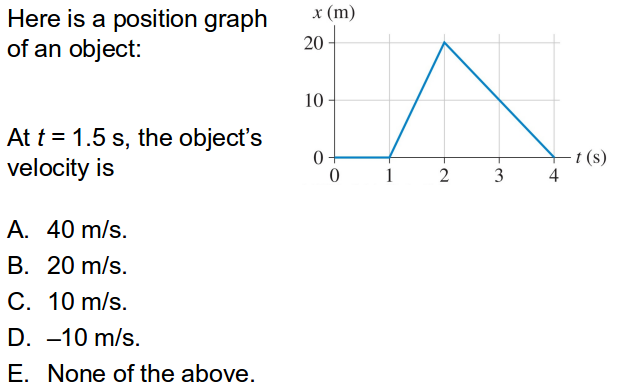
\includegraphics[width=\textwidth]{../figures/QC2_6.png}
\end{center}
\only<2->{\checkL{0.7cm}{5.7cm}}
\end{frame}

\begin{frame}{Quick Check}
\begin{center}
   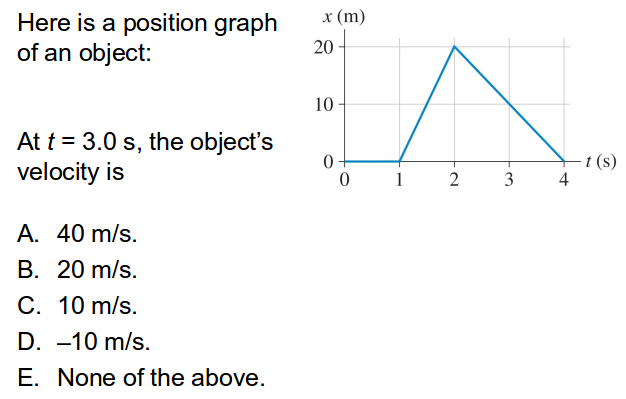
\includegraphics[width=\textwidth]{../figures/QC2_7.png}
\end{center}
\only<2->{\checkL{0.8cm}{6.9cm}}
\end{frame}

\begin{frame}{Quick Check}
\begin{center}
   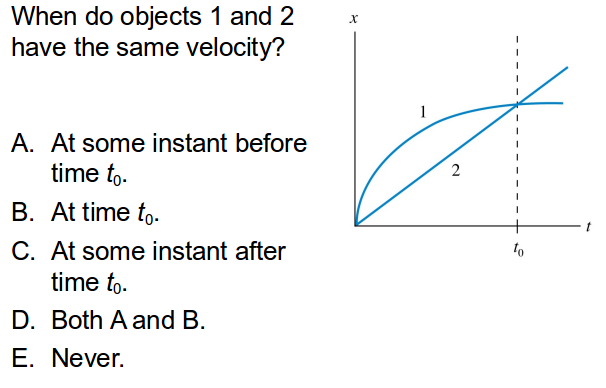
\includegraphics[width=\textwidth]{../figures/QC2_8.png}
\end{center}
\only<2->{\checkL{0.8cm}{3.6cm}
   \begin{textblock*}{\textwidth}(7.1cm,1.6cm) % {block width} (coords)
      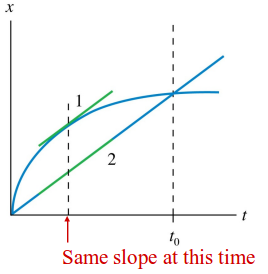
\includegraphics[width=4.8cm]{../figures/QC2_8_2.png}
   \end{textblock*}}
\end{frame}

\begin{frame}{Now Integrals}
\begin{center}
   \color{blue}{\Huge Now Integrals}
\end{center}
\end{frame}

\begin{frame}{Position from Velocity}
\begin{itemize}
   \item Can we use our knowledge of the velocity to predict the position at a future time like we did with the uniform motion equation, $s_f = s_i+v_s\Delta t$?
   \item<2-> Let's start by breaking up a $v(t)$ curve into $N$ steps.
\end{itemize}
\uncover<2>{
\begin{columns}
\begin{column}{0.2\textwidth}
   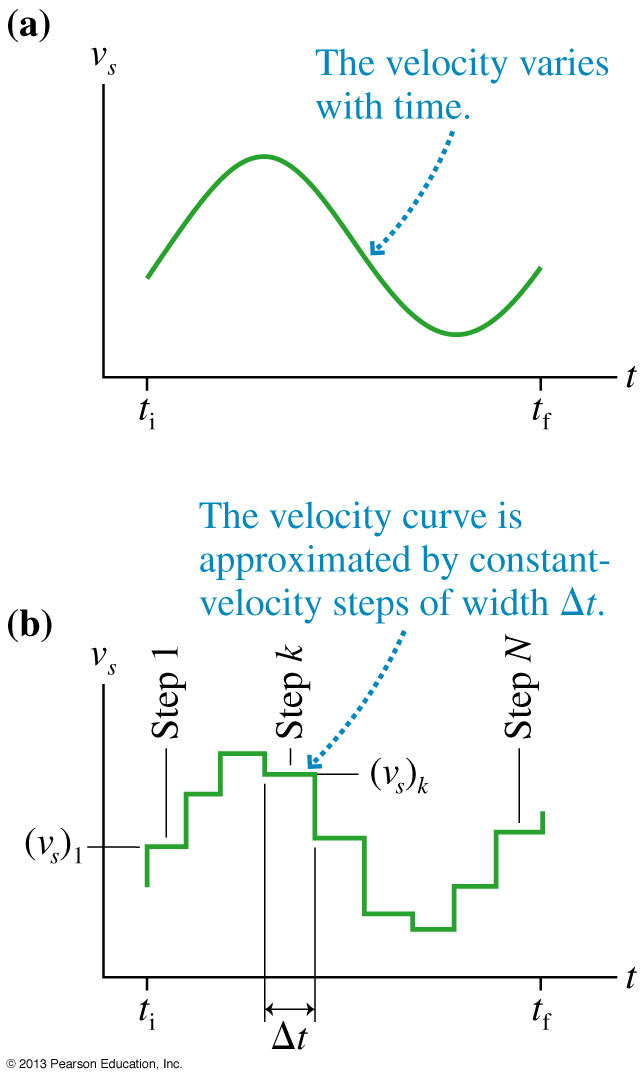
\includegraphics[width=1.4\textwidth]{../figures/02_15_Figure.jpg}
\end{column}
\begin{column}{0.8\textwidth}
   \begin{itemize}
      \item Notice that the motion at each step is uniform motion so we can use ol' faithful, $s_f = s_i + v_s \Delta t \rightarrow \Delta s = v_s \Delta t$.
      \item<3-> So $v_s(t_k)\Delta t$ is the amount that is moved during between the steps $k$ and $k+1$.
      \item<4-> So if I want $\Delta s = s_f - s_i$ then I want to sum over all of steps, $\Delta s \approx \Delta s_1 + \Delta s_2 + \ldots + \Delta s_N = \sum\limits_{k=1}^N (v_s)_k\Delta t$.
   \end{itemize}
\end{column}
\end{columns}}
\end{frame}

\begin{frame}{Position from Velocity}
\begin{columns}
\begin{column}{0.3\textwidth}
   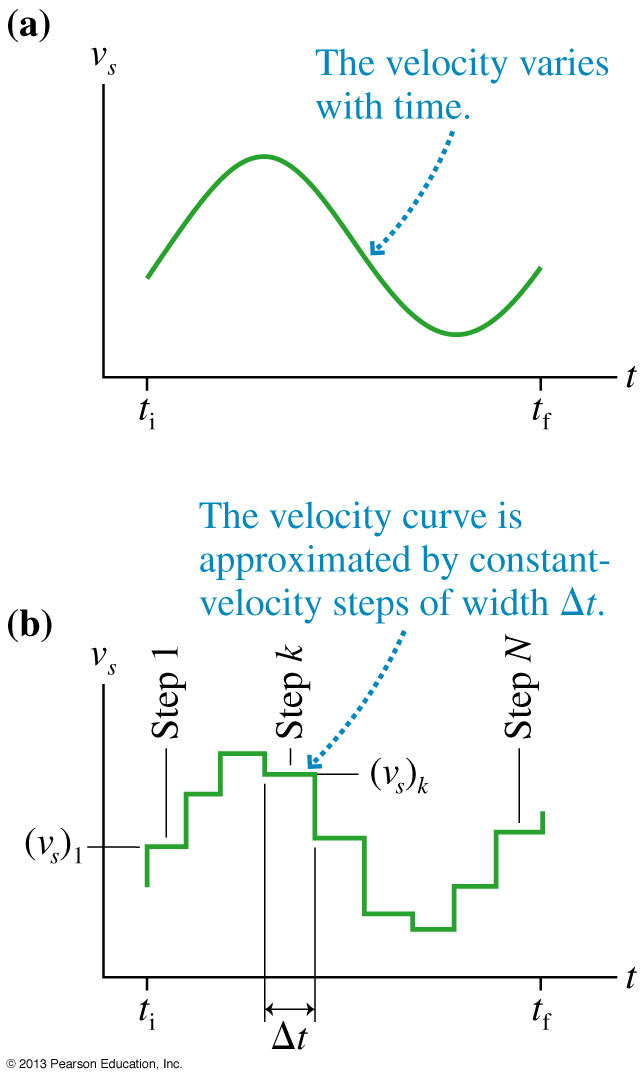
\includegraphics[width=\textwidth]{../figures/02_15_Figure.jpg}
\end{column}
\begin{column}{0.7\textwidth}
   \begin{itemize}
      \item We can then take this and from it determine the final position of a particle if we know it's initial position, $s_i$ and it's velocity at each time, $v(t)$.
      \begin{equation*}
         s_f \approx s_i + \sum\limits_{k=1}^N (v_s)_k\Delta t
      \end{equation*}
      \item<2-> How do we get rid of the pesky approximate sign ($\approx$) though because we can't the true answer?
      \uncover<3>{\begin{shaded}
      \begin{equation}
         s_f = s_i + \lim\limits_{\Delta t \rightarrow 0} \sum\limits_{k=1}^N (v_s)_k\Delta t = s_i + \int\limits_{t_i}^{t_f}v_s dt
         \label{eq:integral}
      \end{equation}
      \end{shaded}}
   \end{itemize}
\end{column}
\end{columns}
\end{frame}

\begin{frame}{Position from Velocity}
\begin{itemize}
   \item Just like we had a geometrical definition for a derivative let's find one for integrals.
   \uncover<2>{\begin{center}
      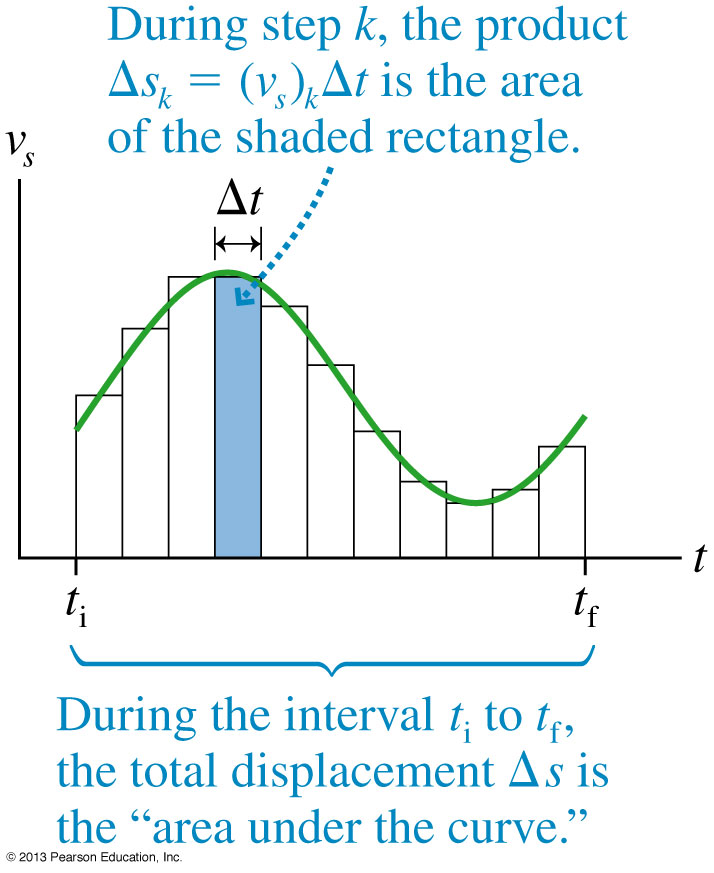
\includegraphics[width=0.3\textwidth]{../figures/02_16_Figure.jpg}
      \uncover<3>{\begin{shaded}
      \begin{equation}
         s_f = s_i + \text{area under the velocity curve } v_s \text{ between } t_i \text{ and } t_f
      \end{equation}
      \end{shaded}}
   \end{center}}
\end{itemize}
\end{frame}

\begin{frame}{Quick Check}
\begin{center}
   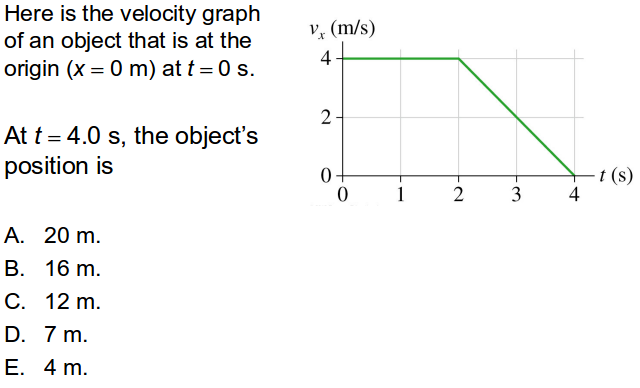
\includegraphics[width=\textwidth]{../figures/QC2_9.png}
\end{center}
\only<2->{\checkL{0.8cm}{6.3cm}}
\end{frame}

\begin{frame}{Quick Check}
\begin{center}
   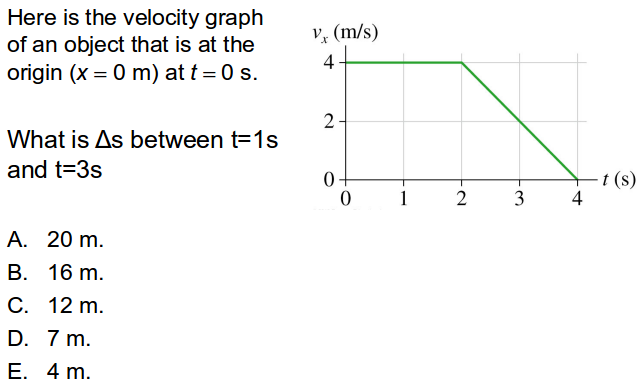
\includegraphics[width=\textwidth]{../figures/QC2_9_2.png}
\end{center}
\only<2->{\checkL{0.8cm}{6.8cm}}
\end{frame}

\begin{frame}{Integrals Review}
\begin{itemize}
   \item Again let's look at integrating polynomials. Think of undoing a derivative (multiply by power and subtract 1 from power).
   \begin{equation*}
      \int\limits_{t_i}^{t_f} ct^ndt = \uncover<2>{\frac{ct^{n+1}}{n+1}\bigg|_{t_i}^{t_f} = \frac{ct_f^{n+1}}{n+1} - \frac{ct_i^{n+1}}{n+1} ~~~~~ (n \ne -1)}
   \end{equation*}
   \uncover<3>{
      \item Here is another identity for integrals
   \begin{equation*}
      \int\limits_{t_i}^{t_f} (u(t)+w(t))dt = \int\limits_{t_i}^{t_f} u(t)dt + \int\limits_{t_i}^{t_f} w(t)dt
   \end{equation*}}
\end{itemize}
\end{frame}

\begin{frame}{Quick Check}
\begin{center}
   From the v(t) graph find the position of this particle at time $t$.
   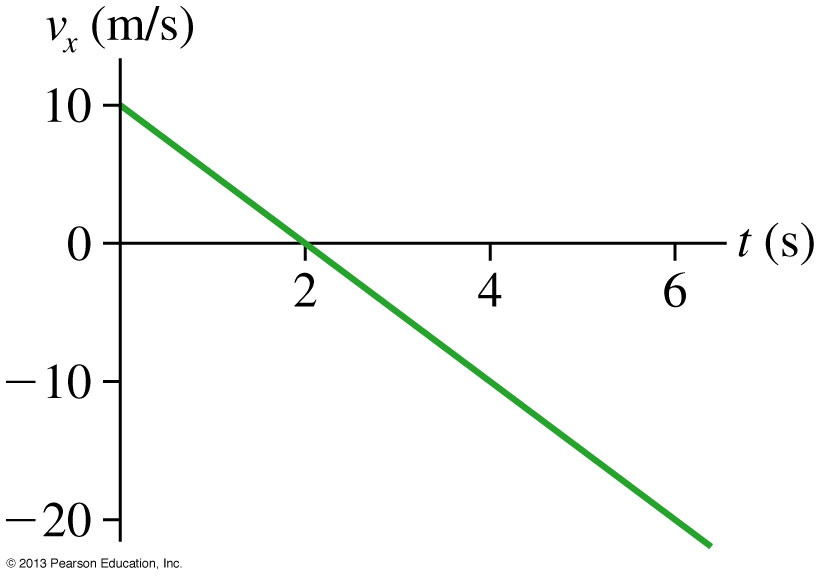
\includegraphics[width=0.5\textwidth]{../figures/02_18_Figure.jpg}
\end{center}
\begin{itemize}
   \item<2-> The first step might be to figure out v(t), v(t)=10-5t (where t is in seconds and v is in m/s).
\end{itemize}
\end{frame}

\begin{frame}{Position from Velocity}
\begin{center}
   $v(t) = 10-5t$ and $x(t=0)=30m$
\end{center}
\begin{itemize}
   \item Then you might plug $v(t)$ and your initial conditions into the equation $s_f = s_i + \int\limits_{t_i}^{t_f}v_sdt$.
   \begin{align*}
      \uncover<2>{x&=x_i+\int\limits_0^t v(t) dt = 30 \text{ m } + \int\limits_0^t(10-5t)dt} \\
      \uncover<3>{&= 30 \text{ m } + \int\limits_0^t 10~dt - \int\limits_0^t 5t~dt} \\
      \uncover<4>{&= 30 \text{ m } + 10t\bigg|_0^t - \frac{5}{2}t^2\bigg|_0^t} \\
      \uncover<5>{&= 30 \text{ m } + (10t-10*0) - \left(\frac{5}{2}t^2-\frac{5}{2}0^2\right)} \\
      \uncover<6>{x&= 30 \text{ m } + 10t - \frac{5}{2}t^2} \\
   \end{align*}
\end{itemize}
\end{frame}

\begin{frame}{Motion with Constant Acceleration}
\begin{center}
   \color{blue}{\Huge Motion with Constant Acceleration}
\end{center}
\end{frame}

\begin{frame}{Motion with Constant Acceleration}
\begin{itemize}
   \item {\bf Acceleration}: Accleration is the rate at which velocity changes.
   \item The SI units for acceleration are (m/s)/s or m/s$^2$.
   \item<2-> If my velocity is 5m/s and I accelerate at $a=2$m/s$^2$ for 1 second what is my new velocity?
   \begin{itemize} 
      \item<3-> $v=7$m/s 
   \end{itemize}
   \item<4> What about after 2 seconds?
   \begin{itemize} \item<5-> $v=9$m/s \end{itemize}
   \item<6> What $a=-2$m/s$^2$ for 2 seconds?
   \begin{itemize} \item<7-> $v=1$m/s \end{itemize}
\end{itemize}
\end{frame}

\begin{frame}{Motion with Constant Acceleration}
\begin{itemize}
   \item Just like the average velocity the {\bf average acceleration} is the slope of v(t).
   \begin{equation*}
      a_{ave} = \frac{\Delta v}{\Delta t}
   \end{equation*}
   \uncover<2>{
   \item If the acceleration is constant then $a_{ave}$ and the instantaneous acceleration, $a_s$ are the same.
   \begin{equation*}
      a_{s} = \frac{dv}{dt}
   \end{equation*}
   }
\end{itemize}
\end{frame}

\begin{frame}{Quick Check}
\begin{center}
   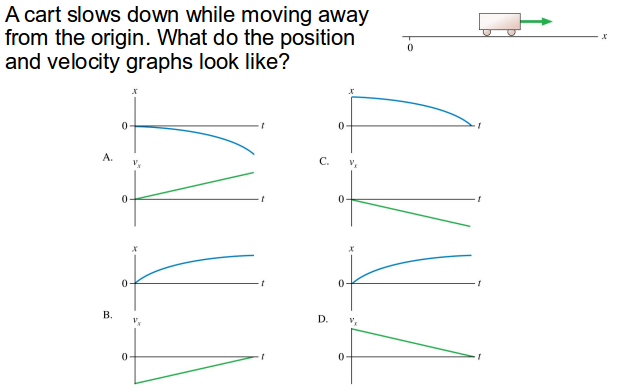
\includegraphics[width=\textwidth]{../figures/QC2_11.png}
\end{center}
\only<2->{\checkL{6.0cm}{6.4cm}}
\end{frame}

\begin{frame}{Quick Check}
\begin{center}
   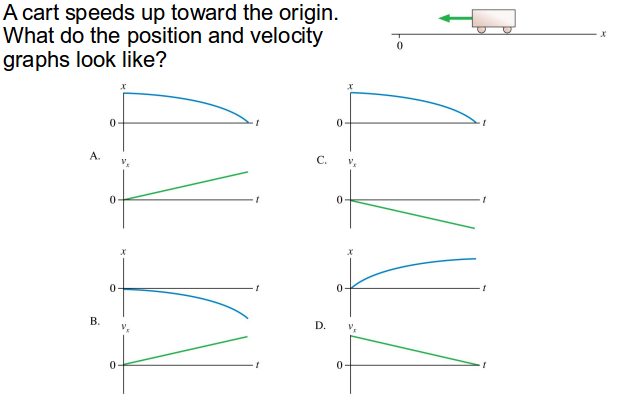
\includegraphics[width=\textwidth]{../figures/QC2_12.png}
\end{center}
\only<2->{\checkL{6.0cm}{3.7cm}}
\end{frame}

\begin{frame}{Quick Check}
\begin{center}
   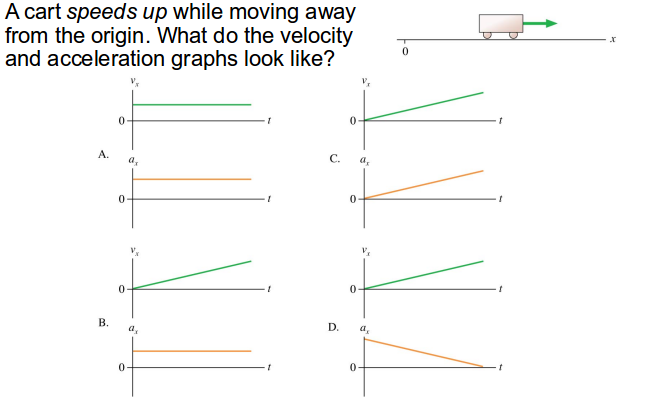
\includegraphics[width=\textwidth]{../figures/QC2_14.png}
\end{center}
\only<2->{\checkL{2.2cm}{6.4cm}}
\end{frame}

\begin{frame}{Quick Check}
\begin{center}
   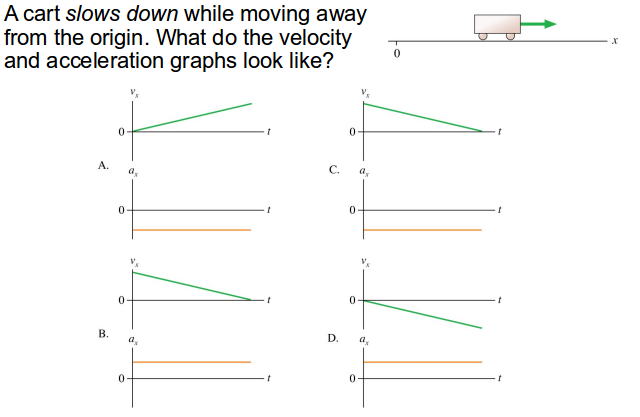
\includegraphics[width=\textwidth]{../figures/QC2_15.png}
\end{center}
\only<2->{\checkL{6.2cm}{3.8cm}}
\end{frame}

\begin{frame}{Quick Check}
\begin{center}
   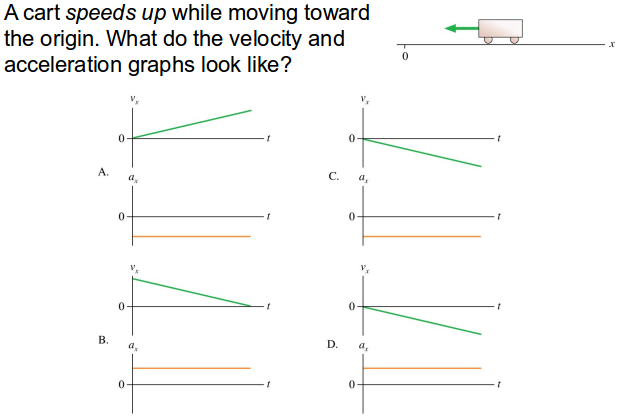
\includegraphics[width=\textwidth]{../figures/QC2_16.png}
\end{center}
\only<2->{\checkL{6.2cm}{3.8cm}}
\end{frame}

\begin{frame}{Kinematic Equations}
\begin{itemize}
   \item Remember with the initial position and the velocity we could calculation the positon with $s_f = s_i + \int\limits_{t_i}^{t_f} v_s dt$
   \item Since we know that the acceleration is the slope of $v(t)$, $a_{ave}=\frac{\Delta v}{\Delta t} \rightarrow v(t) = v_i + a\Delta t$ we can plug this into the integral.
   \item<2-> Practice your integration by plugging v(t) into the integral above to find an expression for the positon $s(t)$ in terms of the initial velocity and the acceleration.
   \begin{equation*}
      s_f = s_i + v_i\Delta t + \frac{1}{2}a(\Delta t)^2
   \end{equation*}
\end{itemize}
\end{frame}

\begin{frame}{Kinematic Equations}
\begin{itemize}
   \item If a particle is initially at $s_i$ with a velocity of $v_i$ you can figure out what the final velocity is by substituting in $\Delta t = \Delta v/a$ into the previous equation. This gives us the third kinematic equation.
\end{itemize}
\begin{center}
\begin{shaded}
\begin{align}
   v_f &= v_i + a\Delta t \\
   s_f &= s_i + v_i\Delta t + \frac{1}{2}a(\Delta t)^2 \\
   v_f^2 &= v_i^2 + 2a\Delta s
\end{align}
\end{shaded}
\end{center}
\end{frame}

\begin{frame}{Kinetmatic Equations - Practice}
   A rocket sled accelerates at 50 m/s$^2$ for 5.0 s, coasts for 3.0 s, then deploys a braking parachute and accelerated at -3.0 m/s$^2$ (you would call this deceleration) until it comes to a stop.
\begin{enumerate}[a.]
   \item What is the maximum velocity of the rocket sled?
   \item What is the total distance traveled?
\end{enumerate}
\uncover<2>{
\begin{center}
   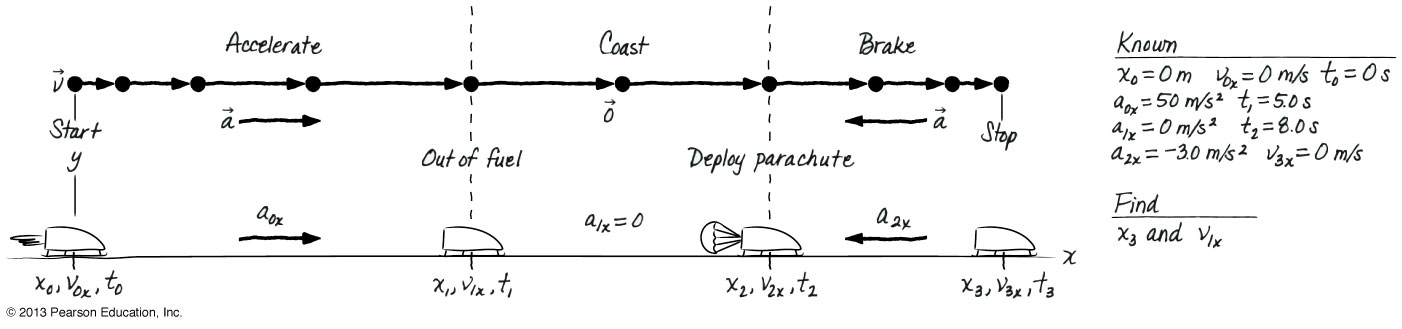
\includegraphics[width=\textwidth]{../figures/02_25_Figure.jpg}
   \uncover<3>{\\ $v_{1x}=250$ m/s \\ $x_3=12000$ m}
\end{center}}
\end{frame}

\begin{frame}{Picture References}
\tiny
Nothing this time
\end{frame}

\end{document}
